\documentclass[12pt,a4paper]{article}

% ── Geometry & Spacing ──
\usepackage[margin=1in]{geometry}
\usepackage{setspace}
\onehalfspacing
\setlength{\headheight}{14.5pt}
\addtolength{\topmargin}{-2.5pt}
\setlength{\parskip}{2pt}

% ── Fonts (Times New Roman equivalent) ──
\usepackage[utf8]{inputenc}
\usepackage[T1]{fontenc}
\usepackage{mathptmx}

% ── Colors & Graphics ──
\usepackage[dvipsnames,svgnames,x11names]{xcolor}
\usepackage{graphicx}
\usepackage{float}
\usepackage{caption}
\usepackage{subcaption}
\captionsetup{font=small}

% ── Links ──
\usepackage[colorlinks=true,linkcolor=NavyBlue,urlcolor=RoyalBlue]{hyperref}

% ── Lists & Tables ──
\usepackage{enumitem}
\usepackage{booktabs}
\usepackage{tabularx}
\usepackage{colortbl}

% ── Section Colors ──
\usepackage{titlesec}
\definecolor{sectionblue}{HTML}{1A3A5C}
\definecolor{subsecblue}{HTML}{2E6B8A}
\definecolor{accentcyan}{HTML}{00BCD4}
\definecolor{softbg}{HTML}{F0F6FA}
\definecolor{alertred}{HTML}{C0392B}
\definecolor{successgreen}{HTML}{27AE60}
\definecolor{warnorg}{HTML}{E67E22}
\definecolor{darkbg}{HTML}{0D1B2A}

\titleformat{\section}
  {\normalfont\Large\bfseries\color{sectionblue}}
  {\thesection.}{0.5em}{}[\color{accentcyan}\titlerule]
\titlespacing*{\section}{0pt}{10pt}{6pt}

\titleformat{\subsection}
  {\normalfont\large\bfseries\color{subsecblue}}
  {\thesubsection}{0.5em}{}
\titlespacing*{\subsection}{0pt}{8pt}{4pt}

% ── Header / Footer ──
\usepackage{fancyhdr}
\pagestyle{fancy}
\fancyhf{}
\fancyhead[L]{\small\color{sectionblue}\textbf{Project Vulner}}
\fancyhead[R]{\small\color{sectionblue}Progress Report}
\fancyfoot[C]{\small\color{gray}\thepage}
\renewcommand{\headrulewidth}{0.8pt}
\renewcommand{\headrule}{\hbox to \headwidth{\color{accentcyan}\leaders\hrule height \headrulewidth\hfill}}

% ── Colored Boxes ──
\usepackage[most]{tcolorbox}

\newtcolorbox{infobox}[1][]{
  colback=softbg, colframe=accentcyan, coltitle=white,
  fonttitle=\bfseries, title=#1, rounded corners,
  boxrule=1pt, left=4pt, right=4pt, top=2pt, bottom=2pt
}

\newtcolorbox{challengebox}[1][]{
  colback=red!3, colframe=alertred!70, coltitle=white,
  fonttitle=\bfseries, title=#1, rounded corners,
  boxrule=1pt, left=4pt, right=4pt, top=2pt, bottom=2pt
}

\newtcolorbox{successbox}[1][]{
  colback=green!3, colframe=successgreen!70, coltitle=white,
  fonttitle=\bfseries, title=#1, rounded corners,
  boxrule=1pt, left=4pt, right=4pt, top=2pt, bottom=2pt
}

% ══════════════════════════════════════════════════
\begin{document}

% ── TITLE HEADER ──
\begin{center}
\colorbox{darkbg}{%
\parbox{0.88\textwidth}{%
\centering
\vspace{0.4cm}
{\LARGE\bfseries\color{accentcyan} Project Vulner}\\[0.2cm]
{\large\color{white} Cybersecurity Vulnerability Detection Platform}\\[0.12cm]
{\small\color{gray!60}\rule{0.4\textwidth}{0.4pt}}\\[0.12cm]
{\normalsize\color{white} Project Progress Report --- April 2026}
\vspace{0.35cm}
}}
\end{center}
\vspace{0.3cm}

% ══════════════════════════════════════════════════
\section{Project Overview}

Project Vulner is an enterprise-grade SaaS cybersecurity platform providing \textbf{automated vulnerability detection} through intelligent code analysis. Developers and security teams submit raw source code or entire Git repository URLs; the platform processes submissions asynchronously and returns comprehensive vulnerability assessments enriched with AI-based confidence metrics. The system supports scanning across multiple languages including C/C++, Python, JavaScript, Java, C\#, Go, Ruby, and PHP.

\begin{infobox}[Core Technology Stack]
\begin{itemize}[noitemsep,leftmargin=*]
  \item \textcolor{RoyalBlue}{\textbf{Frontend:}} Next.js 16 / React 19 with Tailwind CSS, Framer Motion, Three.js
  \item \textcolor{successgreen}{\textbf{Backend:}} ASP.NET Core 9 Web API --- 4-layer DDD (Domain, Application, Infrastructure, API)
  \item \textcolor{Plum}{\textbf{AI Engine:}} Python FastAPI microservice for vulnerability classification
  \item \textcolor{warnorg}{\textbf{Data \& Jobs:}} SQL Server with EF Core; Hangfire for persistent background processing
\end{itemize}
\end{infobox}

\begin{figure}[H]
\centering
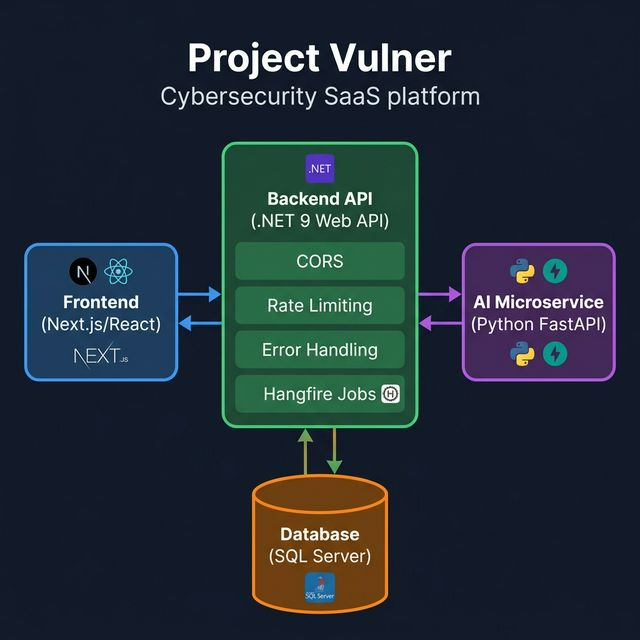
\includegraphics[width=0.52\textwidth]{fig_architecture.png}
\caption{Three-tier system architecture showing the Next.js frontend, .NET 9 backend with middleware pipeline, Python FastAPI AI service, and SQL Server persistence layer.}
\label{fig:arch}
\end{figure}

% ══════════════════════════════════════════════════
\section{Work Completed}

\subsection{Backend API and Database}
The server-side foundation uses ASP.NET Core 9 partitioned into four architectural layers enforcing strict separation of concerns. The \texttt{CodeScan} entity tracks scan ID (GUID), type (Code/RepoUrl), submitted payload, branch, status lifecycle (\textit{Pending}~$\to$~\textit{Running}~$\to$~\textit{Completed\,$|$\,Failed}), vulnerability flag, AI confidence score, raw JSON response, and creation timestamp.

\subsection{Background Processing with Hangfire}
Repository cloning and file-by-file AI inference are delegated to \textbf{Hangfire} background jobs backed by SQL Server. The \texttt{CodeScanJob} orchestrates Git clone operations via LibGit2Sharp, extracts source files by extension (with 1\,MB per-file and 100\,MB per-repo caps), dispatches each to the AI endpoint, and aggregates results.

\begin{figure}[H]
\centering
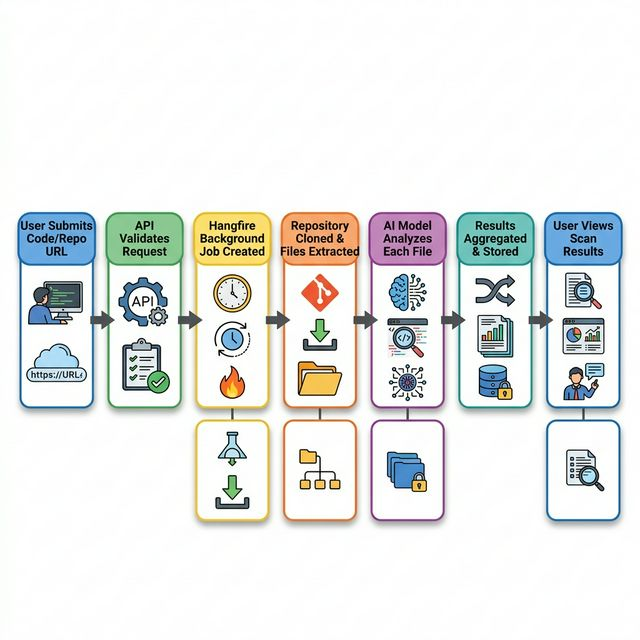
\includegraphics[width=0.72\textwidth]{fig_workflow.png}
\caption{End-to-end scanning workflow: user submission, validation, background job, repository cloning, AI analysis, result aggregation, and final reporting.}
\label{fig:workflow}
\end{figure}

\subsection{AI Microservice and Security Middleware}
An isolated Python FastAPI service exposes \texttt{POST /scan} for vulnerability classification. The .NET \texttt{AiScanner} client uses \texttt{HttpClientFactory} with Polly policies (3-retry exponential backoff, 60s timeout).

\begin{successbox}[Implemented Security Layers]
\begin{enumerate}[noitemsep,leftmargin=*]
  \item \textbf{CORS Policy} --- Whitelisted frontend origins with explicit header/method grants
  \item \textbf{Global Error Handler} --- Converts exceptions to consistent JSON responses with trace IDs
  \item \textbf{Rate Limiting} --- 10 req/min and 100 req/hour per IP (HTTP 429 response)
  \item \textbf{Input Validation} --- Max 100{,}000 characters for code; 100\,MB repository cap; 1\,MB file cap
\end{enumerate}
\end{successbox}

\subsection{Frontend Interface}
The client-side application was built with Next.js 16 and React 19, featuring a cybersecurity-themed landing page with particle effects, animated 3D elements via Three.js, and glassmorphism card designs.

\begin{figure}[H]
\centering
\begin{subfigure}[b]{0.47\textwidth}
  \centering
  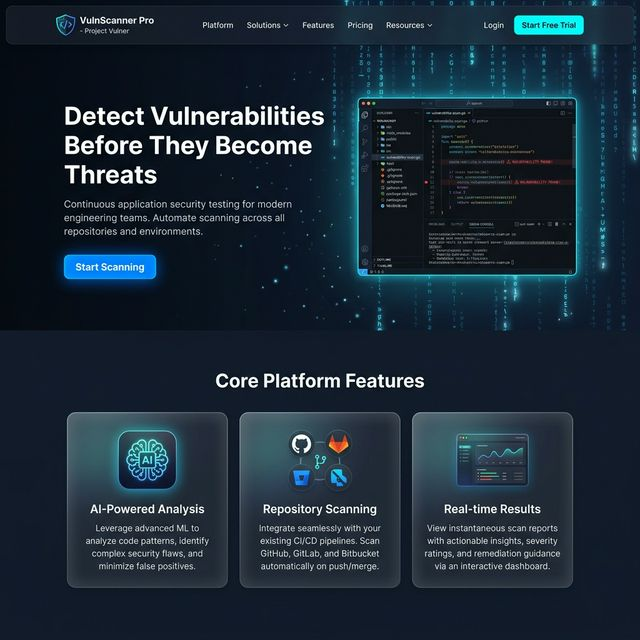
\includegraphics[width=\textwidth]{fig_frontend.png}
  \caption{Landing page with cyber-themed hero}
\end{subfigure}
\hfill
\begin{subfigure}[b]{0.47\textwidth}
  \centering
  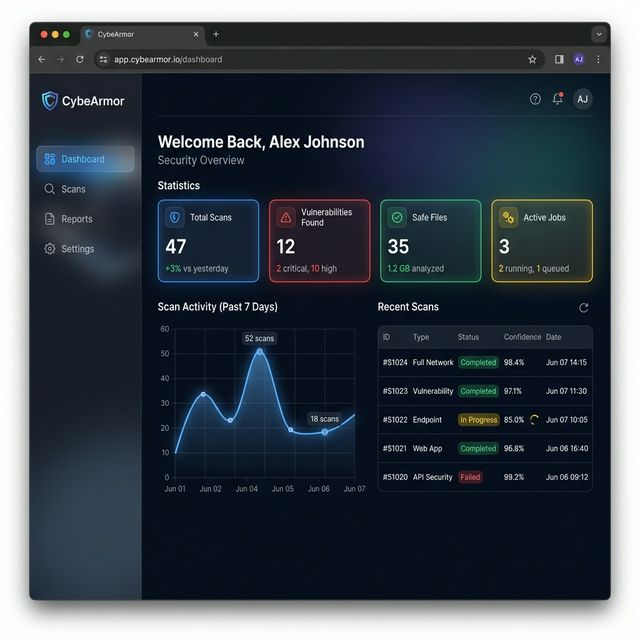
\includegraphics[width=\textwidth]{fig_dashboard.png}
  \caption{Dashboard with scan analytics}
\end{subfigure}
\caption{Project Vulner web application: (a) animated landing page and (b) admin dashboard with statistics tab.}
\label{fig:screens}
\end{figure}

% ══════════════════════════════════════════════════
\section{Challenges Faced}

\begin{challengebox}[Challenge 1: Cross-Origin Network Failures]
Frontend requests were rejected with 403 errors due to missing CORS headers. \textcolor{successgreen}{\textbf{Fix:}} Explicit CORS profiles in \texttt{Program.cs} whitelisting frontend origins; AI service configured for backend-only access.
\end{challengebox}

\begin{challengebox}[Challenge 2: Repository Timeout Cascades]
Large repos caused cumulative timeouts during sequential AI inference calls. \textcolor{successgreen}{\textbf{Fix:}} Granular per-file operations with 60s individual timeouts, repository-level size caps, and Polly retry policies to absorb transient failures.
\end{challengebox}

\begin{challengebox}[Challenge 3: Inconsistent AI Output Structure]
Unpredictable JSON structures from the AI model caused deserialization crashes. \textcolor{successgreen}{\textbf{Fix:}} A generic \texttt{ServiceResult<T>} wrapper guarantees uniform response envelopes; strict TypeScript interfaces and C\# records ensure end-to-end type safety.
\end{challengebox}

% ══════════════════════════════════════════════════
\section{Work in Progress}

Two parallel development tracks are currently active:
\begin{enumerate}[leftmargin=*,noitemsep]
  \item \textbf{Differential Scanning} --- Expanding \texttt{ICodeScanService} to skip unmodified files based on Git commit hashes, reducing redundant AI inference calls.
  \item \textbf{Dashboard Components} --- Building \texttt{AllScansTable} (sortable/filterable), \texttt{ScanFilters} (severity filtering), and \texttt{ScanDetails} modal panels with per-file drilldown views.
\end{enumerate}

\begin{figure}[H]
\centering
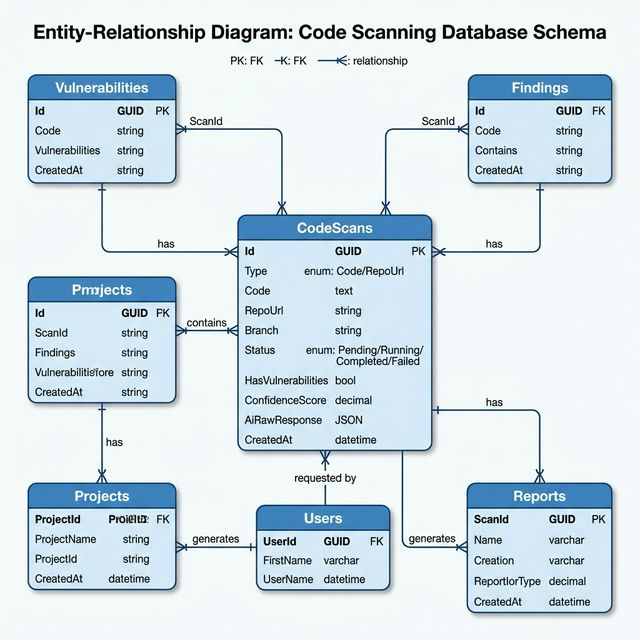
\includegraphics[width=0.58\textwidth]{fig_database.png}
\caption{Entity-Relationship diagram of the code scanning database centered on the \texttt{CodeScans} table.}
\label{fig:erd}
\end{figure}

% ══════════════════════════════════════════════════
\section{Next Steps}

\begin{table}[H]
\centering \small
\rowcolors{2}{softbg}{white}
\begin{tabularx}{0.95\textwidth}{l X l}
\toprule
\rowcolor{sectionblue}\textcolor{white}{\textbf{Priority}} & \textcolor{white}{\textbf{Task}} & \textcolor{white}{\textbf{Phase}} \\
\midrule
\textcolor{alertred}{\textbf{High}} & JWT authentication with RBAC (Admin/User) & II \\
\textcolor{alertred}{\textbf{High}} & Cursor-based pagination for scan endpoints & II \\
\textcolor{warnorg}{\textbf{Medium}} & Docker containerization via \texttt{docker-compose} & II \\
\textcolor{warnorg}{\textbf{Medium}} & CI/CD pipeline with GitHub Actions & III \\
\textcolor{RoyalBlue}{\textbf{Low}} & Comprehensive unit and integration test suites & III \\
\bottomrule
\end{tabularx}
\caption{Prioritized development roadmap for upcoming project phases.}
\end{table}

% ══════════════════════════════════════════════════
\section{Team Contribution}

\begin{table}[H]
\centering \small
\rowcolors{2}{softbg}{white}
\begin{tabularx}{0.95\textwidth}{l X}
\toprule
\rowcolor{sectionblue}\textcolor{white}{\textbf{Role}} & \textcolor{white}{\textbf{Responsibilities}} \\
\midrule
\textcolor{RoyalBlue}{\textbf{Backend Architect}} & .NET 4-layer architecture, EF Core models, Hangfire pipelines, middleware orchestration \\
\textcolor{Plum}{\textbf{AI Engineer}} & FastAPI inference engine, ML model training, inter-service communication protocol \\
\textcolor{accentcyan}{\textbf{Frontend Developer}} & Next.js application, Axios client setup, responsive UI/UX, 3D animations \\
\textcolor{successgreen}{\textbf{QA \& Security}} & CORS testing, rate-limit stress testing, input validation, integration checklist \\
\bottomrule
\end{tabularx}
\caption{Team responsibility matrix.}
\end{table}

\begin{center}
\small\itshape All members participate in cross-functional code reviews and collaborative debugging sessions to maintain holistic system understanding.
\end{center}

\end{document}
